%% abtex2-modelo-artigo.tex, v-1.9.7 laurocesar
%% Copyright 2012-2018 by abnTeX2 group at http://www.abntex.net.br/ 
%%
%% This work may be distributed and/or modified under the
%% conditions of the LaTeX Project Public License, either version 1.3
%% of this license or (at your option) any later version.
%% The latest version of this license is in
%%   http://www.latex-project.org/lppl.txt
%% and version 1.3 or later is part of all distributions of LaTeX
%% version 2005/12/01 or later.
%%
%% This work has the LPPL maintenance status `maintained'.
%% 
%% The Current Maintainer of this work is the abnTeX2 team, led
%% by Lauro César Araujo. Further information are available on 
%% http://www.abntex.net.br/
%%
%% This work consists of the files abntex2-modelo-artigo.tex and
%% abntex2-modelo-references.bib
%%
% ---------------------------------------------------------------
% ---------------------------------------------------------------
% abnTeX2: Modelo de Artigo Acadêmico em conformidade com
% ABNT NBR 6022:2018: Informação e documentação - Artigo em publicação 
% periódica científica - Apresentação
% ---------------------------------------------------------------
% Adaptado para uso na instituição acadêmica Senai Cimatec.
% 25/05/2022
% -----------------------------------------------------------------

\documentclass[
	% -- opções da classe memoir --
	article,			% indica que é um artigo acadêmico
	11pt,				% tamanho da fonte
	oneside,			% para impressão apenas no recto. Oposto a twoside
	a4paper,			% tamanho do papel. 
	% -- opções da classe abntex2 --
	%chapter=TITLE,		% títulos de capítulos convertidos em letras maiúsculas
	%section=TITLE,		% títulos de seções convertidos em letras maiúsculas
	%subsection=TITLE,	% títulos de subseções convertidos em letras maiúsculas
	%subsubsection=TITLE % títulos de subsubseções convertidos em letras maiúsculas
	% -- opções do pacote babel --
	english,			% idioma adicional para hifenização
	brazil,				% o último idioma é o principal do documento
	sumario=tradicional
	]{abntex2}

% Pacotes fundamentais 
\usepackage{lmodern}		% Usa a fonte Latin Modern
\usepackage[T1]{fontenc}	% Selecao de codigos de fonte.
\usepackage[utf8]{inputenc}	% Conversão automática dos acentos
\usepackage{indentfirst}	% Indenta o 1. parágrafo de cada seção.
\usepackage{nomencl} 		% Lista de simbolos
\usepackage{color}			% Controle das cores
\usepackage{graphicx}		% Inclusão de gráficos
\usepackage{microtype} 		% para melhorias de justificação
% ---
\usepackage{lipsum}			% para geração de dummy text
% ---
% Pacotes de citações
\usepackage[brazilian,hyperpageref]{backref}	
\usepackage[alf]{abntex2cite}
% ---
% Configurações do pacote backref
% Usado sem a opção hyperpageref de backref
\renewcommand{\backrefpagesname}{Citado na(s) página(s):~}
\renewcommand{\backref}{}
\renewcommand*{\backrefalt}[4]{
	\ifcase #1 %
		Nenhuma citação no texto.%
	\or
		Citado na página #2.%
	\else
		Citado #1 vezes nas páginas #2.%
	\fi}%
% --- Informações de dados para CAPA e FOLHA DE ROSTO ---
\titulo{Modelo Canônico de Artigo científico com \abnTeX adaptado}
\tituloestrangeiro{}
\autor{
      John Marston\thanks{``Recomenda-se que os dados de vinculação e endereço constem em nota, com sistema de chamada próprio, diferente do sistema adotado para citações no texto.'' \url{http://www.abntex.net.br/}} 
      %\\[0.5cm] 
      Lauro César Araujo\thanks{``Constar currículo sucinto de cada autor, com vinculação corporativa e endereço de contato.''} 
      }
\local{Brasil}
\data{25/05/2022}
% ---
\definecolor{blue}{RGB}{41,5,195}
% ---
% informações do PDF
\makeatletter
\hypersetup{
     	%pagebackref=true,
		pdftitle={\@title}, 
		pdfauthor={\@author},
    	pdfsubject={Modelo de artigo científico com abnTeX2},
	    pdfcreator={LaTeX with abnTeX2},
		pdfkeywords={abnt}{latex}{abntex}{abntex2}{atigo científico}, 
		colorlinks=true,  % false: boxed links; true: colored links
    	linkcolor=blue,   % color of internal links
    	citecolor=blue,   % color of links to bibliography
    	filecolor=magenta,% color of file links
		urlcolor=blue,
		bookmarksdepth=4
}
\makeatother
\makeindex
\setlrmarginsandblock{3cm}{3cm}{*}
\setulmarginsandblock{3cm}{3cm}{*}
\checkandfixthelayout
% ---
\setlength{\parindent}{1.3cm}
\setlength{\parskip}{0.2cm}  
\SingleSpacing
% ----
\begin{document}
\selectlanguage{brazil}
\frenchspacing
% ----------------------------------------------------------
% ELEMENTOS PRÉ-TEXTUAIS
% ----------------------------------------------------------
% Se desejar escrever o artigo em duas colunas, descomente a linha abaixo e a linha com o texto ``FIM DE ARTIGO EM DUAS COLUNAS''.
% \twocolumn[    		% INICIO DE ARTIGO EM DUAS COLUNAS
%
% página de titulo principal (obrigatório)
\maketitle
% titulo em outro idioma (opcional)

% resumo em português
\begin{resumoumacoluna}
	Conforme a ABNT NBR 6022:2018, o resumo no idioma do documento é elemento obrigatório.
	Constituído de uma sequência de frases concisas e objetivas e não de uma simples enumeração de tópicos, não ultrapassando 250 palavras, seguido, logo abaixo, das palavras representativas do conteúdo do trabalho, isto é palavras-chave e/ou descritores, conforme a NBR 6028. (\ldots)
	As palavras-chave devem figurar logo abaixo do resumo, antecedidas da expressão Palavras-chave:, separadas entre si por ponto e finalizadas também por ponto.

	\vspace{\onelineskip}

	\noindent
	\textbf{Palavras-chave}: latex. abntex. editoração de texto.
\end{resumoumacoluna}

% resumo em inglês
\renewcommand{\resumoname}{Abstract}
\begin{resumoumacoluna}
	\begin{otherlanguage*}{english}
		According to ABNT NBR 6022:2018, an abstract in foreign language is optional.

		\vspace{\onelineskip}

		\noindent
		\textbf{Keywords}: latex. abntex.
	\end{otherlanguage*}
\end{resumoumacoluna}

% ]  				% FIM DE ARTIGO EM DUAS COLUNAS
% ----------------------------------------------------------
% ELEMENTOS TEXTUAIS
% ----------------------------------------------------------
\textual
%
\section{Introdução}

Este documento e seu código-fonte são exemplos de referência de uso da classe
\textsf{abntex2} e do pacote \textsf{abntex2cite}. O documento exemplifica a
elaboração de publicação periódica científica impressa produzida conforme a ABNT
NBR 6022:2018 \emph{Informação e documentação - Artigo em publicação periódica
    científica - Apresentação}.

A expressão ``Modelo canônico'' é utilizada para indicar que \abnTeX\ não é
modelo específico de nenhuma universidade ou instituição, mas que implementa tão
somente os requisitos das normas da ABNT. Uma lista completa das normas
observadas pelo \abnTeX\ é apresentada em \citeonline{abntex2classe}.

Sinta-se convidado a participar do projeto \abnTeX! Acesse o site do projeto em
\url{http://www.abntex.net.br/}. Também fique livre para conhecer,
estudar, alterar e redistribuir o trabalho do \abnTeX, desde que os arquivos
modificados tenham seus nomes alterados e que os créditos sejam dados aos
autores originais, nos termos da ``The \LaTeX\ Project Public
License''\footnote{\url{http://www.latex-project.org/lppl.txt}}.

Encorajamos que sejam realizadas customizações específicas deste documento.
Porém, recomendamos que ao invés de se alterar diretamente os arquivos do
\abnTeX, distribua-se arquivos com as respectivas customizações. Isso permite
que futuras versões do \abnTeX~não se tornem automaticamente incompatíveis com
as customizações promovidas. Consulte \citeonline{abntex2-wiki-como-customizar}
para mais informações.

Este exemplo deve ser utilizado como complemento do manual da classe
\textsf{abntex2} \cite{abntex2classe}, dos manuais do pacote
\textsf{abntex2cite} \cite{abntex2cite,abntex2cite-alf} e do manual da classe
\textsf{memoir} \cite{memoir}. Consulte o \citeonline{abntex2modelo} para obter
exemplos e informações adicionais de uso de \abnTeX\ e de \LaTeX.


\section{Exemplos de comandos}

\subsection{Margens}

A norma ABNT NBR 6022:2018 não estabelece uma margem específica a ser utilizada
no artigo científico. Dessa maneira, caso deseje alterar as margens, utilize os
comandos abaixo:

\begin{verbatim}
   \setlrmarginsandblock{3cm}{3cm}{*}
   \setulmarginsandblock{3cm}{3cm}{*}
   \checkandfixthelayout
\end{verbatim}

\subsection{Duas colunas}

É comum que artigos científicos sejam escritos em duas colunas. Para isso,
adicione a opção \texttt{twocolumn} à classe do documento, como no exemplo:

\begin{verbatim}
   \documentclass[article,11pt,oneside,a4paper,twocolumn]{abntex2}
\end{verbatim}

É possível indicar pontos do texto que se deseja manter em apenas uma coluna,
geralmente o título e os resumos. Os resumos em única coluna em documentos com
a opção \texttt{twocolumn} devem ser escritos no ambiente
\texttt{resumoumacoluna}:

\begin{verbatim}
   \twocolumn[              % INICIO DE ARTIGO EM DUAS COLUNAS

     \maketitle             % pagina de titulo

     \renewcommand{\resumoname}{Nome do resumo}
     \begin{resumoumacoluna}
        Texto do resumo.
      
        \vspace{\onelineskip}
 
        \noindent
        \textbf{Palavras-chave}: latex. abntex. editoração de texto.
     \end{resumoumacoluna}
   
   ]                        % FIM DE ARTIGO EM DUAS COLUNAS
\end{verbatim}

\subsection{Recuo do ambiente \texttt{citacao}}

Na produção de artigos (opção \texttt{article}), pode ser útil alterar o recuo
do ambiente \texttt{citacao}. Nesse caso, utilize o comando:

\begin{verbatim}
   \setlength{\ABNTEXcitacaorecuo}{1.8cm}
\end{verbatim}

Quando um documento é produzido com a opção \texttt{twocolumn}, a classe
\textsf{abntex2} automaticamente altera o recuo padrão de 4 cm, definido pela
ABNT NBR 10520:2002 seção 5.3, para 1.8 cm.

\section{Cabeçalhos e rodapés customizados}

Diferentes estilos de cabeçalhos e rodapés podem ser criados usando os
recursos padrões do \textsf{memoir}.

Um estilo próprio de cabeçalhos e rodapés pode ser diferente para páginas pares
e ímpares. Observe que a diferenciação entre páginas pares e ímpares só é
utilizada se a opção \texttt{twoside} da classe \textsf{abntex2} for utilizado.
Caso contrário, apenas o cabeçalho padrão da página par (\emph{even}) é usado.

Veja o exemplo abaixo cria um estilo chamado \texttt{meuestilo}. O código deve
ser inserido no preâmbulo do documento.

\begin{verbatim}
%%criar um novo estilo de cabeçalhos e rodapés
\makepagestyle{meuestilo}
  %%cabeçalhos
  \makeevenhead{meuestilo} %%pagina par
     {topo par à esquerda}
     {centro \thepage}
     {direita}
  \makeoddhead{meuestilo} %%pagina ímpar ou com oneside
     {topo ímpar/oneside à esquerda}
     {centro\thepage}
     {direita}
  \makeheadrule{meuestilo}{\textwidth}{\normalrulethickness} %linha
  %% rodapé
  \makeevenfoot{meuestilo}
     {rodapé par à esquerda} %%pagina par
     {centro \thepage}
     {direita} 
  \makeoddfoot{meuestilo} %%pagina ímpar ou com oneside
     {rodapé ímpar/onside à esquerda}
     {centro \thepage}
     {direita}
\end{verbatim}

Para usar o estilo criado, use o comando abaixo imediatamente após um dos
comandos de divisão do documento. Por exemplo:

\begin{verbatim}
   \begin{document}
     %%usar o estilo criado na primeira página do artigo:
     \pretextual
     \pagestyle{meuestilo}
     
     \maketitle
     ...
     
     %%usar o estilo criado nas páginas textuais
     \textual
     \pagestyle{meuestilo}
     
     \chapter{Novo capítulo}
     ...
   \end{document}  
\end{verbatim}

Outras informações sobre cabeçalhos e rodapés estão disponíveis na seção 7.3 do
manual do \textsf{memoir} \cite{memoir}.

\section{Imagens}
%-----------------------------especificar o tamanho------------------------------------------------------------------------------------------
\begin{figure}[htbp]
    \centerline{
        \includegraphics*[scale=1.5]{imagens/fig1.png} 
        }
\caption{Example of a figure caption.}
\label{fig}
\end{figure}
% %-----------------------------imagem emoldurada--------------------------------------------------------------------------------------------
% \begin{figure}[htbp]
%    \centerline{
%        \fbox{\includegraphics*[scale=1.5]{imagens/fig1.png}} 
%        }
% \caption{Example of a figure caption.}
% \label{fig}
% \end{figure}
% %-----------------------------especificar o altura e largura-------------------------------------------------------------------------------
% \begin{figure}[htbp]
%     \centerline{
%         \includegraphics*[width=2cm, height=3cm]{imagens/fig1.png} 
%         }
% \caption{Example of a figure caption.}
% \label{fig}
% \end{figure}
% %-----------------------------setar a mesma largura do texto-------------------------------------------------------------------------------
% \begin{figure}[htbp]
%     \centerline{
%         \includegraphics*[width=\textwidth]{imagens/fig1.png} 
%         }
% \caption{Example of a figure caption.}
% \label{fig}
% \end{figure}
% %-----------------------------imagem inscrita em outra-------------------------------------------------------------------------------------
% \begin{figure}[ht]
%     \includegraphics[scale=1]{example-image-1x1}
%     \centering
%     \llap{\shortstack{%
%             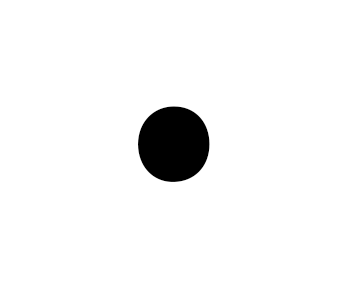
\includegraphics[scale=1.5]{imagens/fig1.png}\\
%             \rule{0ex}{1.3in}%polegadas eixo Y
%           }
%       \rule{0.2in}{0ex}}%polegadas eixo X
%     \caption{This is my embedded figure}
%     \end{figure}
% %-----------------------------4 imagens inscritas em outra---------------------------------------------------------------------------------
% \begin{figure}[ht]
%    \includegraphics[scale=1]{example-image-1x1}
%    \centering
%    %superior esquerda
%    \llap{\shortstack{
%            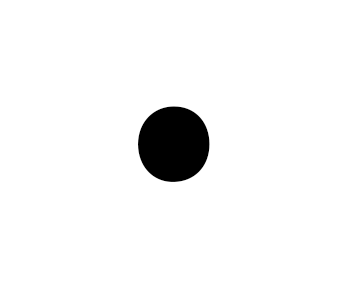
\includegraphics[scale=1.5]{imagens/fig1.png}\\
%            \rule{0ex}{1.35in}%polegadas eixo Y
%          }
%      \rule{1.4in}{0ex}}%polegadas eixo X
%    %inferior esquerda
%    \llap{\shortstack{
%            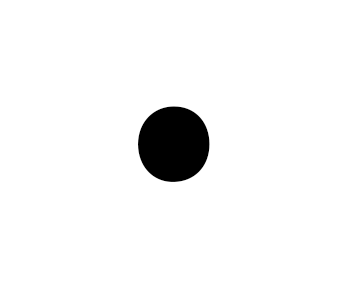
\includegraphics[scale=1.5]{imagens/fig1.png}\\
%            \rule{0ex}{0.15in}%polegadas eixo Y
%         }
%      \rule{1.4in}{0ex}}%polegadas eixo X
%    %superior direita  
%    \llap{\shortstack{
%             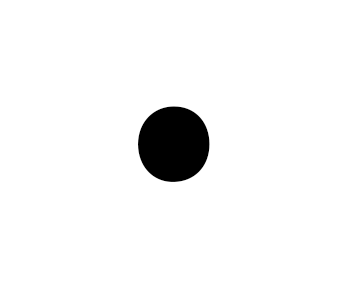
\includegraphics[scale=1.5]{imagens/fig1.png}\\
%             \rule{0ex}{1.35in}%polegadas eixo Y
%          }
%       \rule{0.2in}{0ex}}%polegadas eixo X
%    %inferior direita
%    \llap{\shortstack{
%             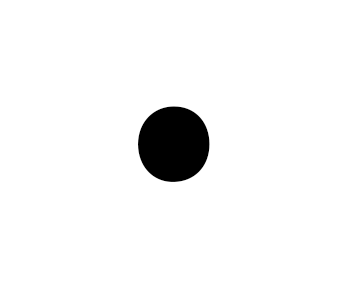
\includegraphics[scale=1.5]{imagens/fig1.png}\\
%             \rule{0ex}{0.15in}%polegadas eixo Y
%          }
%       \rule{0.2in}{0ex}}%polegadas eixo X
%    \caption{This is my embedded figure}
%    \end{figure}
% %-----------------------------sombra na imagem---------------------------------------------------------------------------------------------
% \begin{figure}[htbp]
%    \centerline{
%        \shadowbox{\includegraphics*[scale=1.5]{imagens/fig1.png}} 
%        }
% \caption{Example of a figure caption.}
% \label{fig}
% \end{figure}
%-----------------------------Quebra de texto em torno da figura-----------------------------------------------------------------------------
% Praesent in sapien. Lorem ipsum dolor sit amet, consectetuer adipiscing elit. Duis fringilla tristique neque. Sed interdum libero ut metus. Pellentesque placerat.

% \begin{wrapfigure}{l}{0.25\textwidth}
% 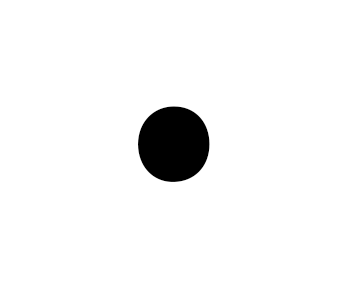
\includegraphics[width=0.9\linewidth]{imagens/fig1.png} 
% \caption{Caption1}
% \label{fig:wrapfig}
% \end{wrapfigure}

% Praesent in sapien. Lorem ipsum dolor sit amet, consectetuer adipiscing elit. Duis fringilla tristique neque. Sed interdum libero ut metus. Pellentesque placerat. Nam rutrum augue a leo. Morbi sed elit sit amet ante lobortis sollicitudin.

% Praesent in sapien. Lorem ipsum dolor sit amet, consectetuer adipiscing elit. Duis fringilla tristique neque. Sed interdum libero ut metus. Pellentesque placerat. Nam rutrum augue a leo. Morbi sed elit sit amet ante lobortis sollicitudin.Praesent in sapien. Lorem ipsum dolor sit amet, consectetuer adipiscing elit. Duis fringilla tristique neque. Sed interdum libero ut metus. Pellentesque placerat. Nam rutrum augue a leo. Morbi sed elit sit amet ante lobortis sollicitudin. Pellentesque placerat. Nam rutrum augue a leo. Morbi sed elit sit amet ante lobortis sollicitudin.mauri.Praesent in sapien. Lorem ipsum dolor sit amet, consectetuer adipiscing elit. Duis fringilla tristique neque. Maecenas dignissim aliquam pellentesque. 

%-----------------------------posição a direita--------------------------------------------------------------------------------------------
% Lorem ipsum dolor sit amet, consectetuer adipiscing elit. Etiam lobortis facilisis sem. Nullam nec mi et neque pharetra sollicitudin.
% \begin{figure}[htbp]
% 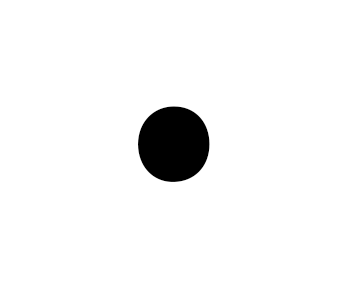
\includegraphics[width=0.3\textwidth, right]{imagens/fig1.png}
% \end{figure}

% Praesent imperdiet mi nec
% ante. Donec ullamcorper, felis non sodales commodo, lectus velit ultrices augue,
% a dignissim nibh lectus placerat pede. Vivamus nunc nunc, molestie ut, ultricies
% vel, semper in, velit. Ut porttitor.

%-----------------------------posição a esquerda--------------------------------------------------------------------------------------------
% Lorem ipsum dolor sit amet, consectetuer adipiscing elit. Etiam lobortis facilisis sem. Nullam nec mi et neque pharetra sollicitudin.
% \begin{figure}[htbp]
% 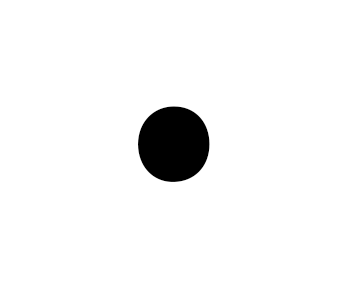
\includegraphics[width=0.3\textwidth]{imagens/fig1.png}
% \end{figure}

% Praesent imperdiet mi nec
% ante. Donec ullamcorper, felis non sodales commodo, lectus velit ultrices augue,
% a dignissim nibh lectus placerat pede. Vivamus nunc nunc, molestie ut, ultricies
% vel, semper in, velit. Ut porttitor.
%-----------------------------2 imagens em 1 figura----------------------------------------------------------------------------------------
% \begin{figure}[h]
   
%    \begin{subfigure}{0.5\textwidth}
%    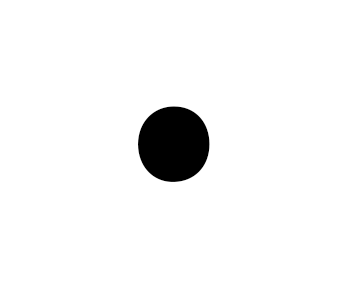
\includegraphics[width=0.9\linewidth, height=6cm]{imagens/fig1.png} 
%    \caption{Caption1}
%    \label{fig:subim1}
%    \end{subfigure}
%    \begin{subfigure}{0.5\textwidth}
%    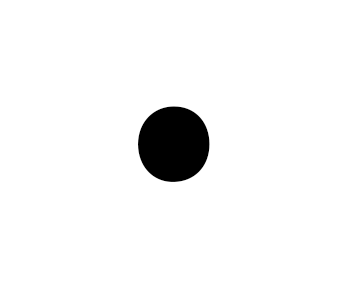
\includegraphics[width=0.9\linewidth, height=6cm]{imagens/fig1.png}
%    \caption{Caption 2}
%    \label{fig:subim2}
%    \end{subfigure}
   
%    \caption{Caption for this figure with two images}
%    \label{fig:image2}
%    \end{figure}
   
\section{Mais exemplos no Modelo Canônico de Trabalhos Acadêmicos}

Este modelo de artigo é limitado em número de exemplos de comandos, pois são apresentados exclusivamente comandos diretamente relacionados com a produção de artigos.

Para exemplos adicionais de \abnTeX\ e \LaTeX, como inclusão de figuras,fórmulas matemáticas, citações, e outros, consulte o documento \citeonline{abntex2modelo}.

\section{Consulte o manual da classe \textsf{abntex2}}

Consulte o manual da classe \textsf{abntex2} \cite{abntex2classe} para uma referência completa das macros e ambientes disponíveis.
\section{Considerações finais}

\lipsum[1]

\begin{citacao}
    \lipsum[2]
\end{citacao}

\lipsum[3]
% ----------------------------------------------------------
\bookmarksetup{startatroot}% Finaliza a parte no bookmark do PDF, para que se inicie o bookmark na raiz 
% ----------------------------------------------------------
% ELEMENTOS PÓS-TEXTUAIS
% ----------------------------------------------------------
\postextual
% 
% Referências bibliográficas
% ----------------------------------------------------------
\bibliography{references}
% 
% Agradecimentos
% ----------------------------------------------------------
\section*{Agradecimentos}
Texto sucinto aprovado pelo periódico em que será publicado. Último elemento pós-textual.
%
\end{document}
